%%
%% Learning from AI-Assisted Developer Workflows
%% Converted to ACM sigconf format
%%
\documentclass[sigconf]{acmart}

%%
%% \BibTeX command to typeset BibTeX logo in the docs
\AtBeginDocument{%
  \providecommand\BibTeX{{%
    Bib\TeX}}}

%% Rights management information
\setcopyright{acmlicensed}
\copyrightyear{2025}
\acmYear{2025}
\acmDOI{XXXXXXX.XXXXXXX}

%% Conference information
\acmConference[Conference acronym 'XX]{Make sure to enter the correct
  conference title from your rights confirmation email}{Month DD--DD,
  2025}{City, Country}
\acmISBN{978-1-4503-XXXX-X/2025/XX}

%%
%% Additional packages needed for the paper
\usepackage{tikz}
\usetikzlibrary{arrows.meta, positioning}
\usepackage[table]{xcolor}
\usepackage{tabularx}
\usepackage{array}

%%
%% end of the preamble, start of the body of the document source.
\begin{document}

%%
%% The "title" command has an optional parameter,
%% allowing the author to define a "short title" to be used in page headers.
\title{Tracing Your Steps: Learning from AI-Assisted Developer Workflows}

%%
%% The "author" command and its associated commands are used to define
%% the authors and their affiliations.
\author{Hamidah Oderinwale}
\email{hamidah.oderinwale@mail.mcgill.ca}
\affiliation{%
  \institution{Your Institution}
  \city{City}
  \state{State}
  \country{Country}
}

%%
%% By default, the full list of authors will be used in the page
%% headers. Often, this list is too long, and will overlap
%% other information printed in the page headers. This command allows
%% the author to define a more concise list
%% of authors' names for this purpose.
\renewcommand{\shortauthors}{Oderinwale}

%%
%% The abstract is a short summary of the work to be presented in the
%% article.
\begin{abstract}
AI-augmented programming has become ubiquitous, with developers increasingly working through iterative, prompt-driven interactions with code generation systems. While recent training paradigms have begun to incorporate developer traces, three fundamental gaps remain: (1) we lack a principled identification of what signals in real workflows are actually learnable and valuable, (2) we do not yet understand how those signals should be used to evaluate and improve code agents, and (3) we have no representation layer that makes raw IDE telemetry comparable, shareable, and governable at scale.

We argue that the next generation of AI evaluation must move from static benchmarks to \emph{in-vivo} measurement of real developer--agent workflows. To that end, we introduce a companion system that captures fine-grained Cursor telemetry and propose representation dimensions that transform raw logs into structured abstractions---files, motifs, and context flows---that enable \emph{evals in the wild}. These representations make it possible to measure, compare, and optimize how software is produced, not just what code is output. The framework enables bidirectional alignment: aligning AI systems to developer needs (matching models to tasks based on workflow patterns) and aligning developers to AI capabilities (revealing which strategies work effectively). Throughout, developers retain agency over data sharing and abstraction levels, maintaining control over how their workflows are represented and analyzed. We outline how this substrate supports personalization, collective learning, and governance of AI-assisted software engineering.
\end{abstract}

%%
%% The code below should be generated by the tool at http://dl.acm.org/ccs.cfm.
%% Please generate the correct terms for your paper.
%%
\begin{CCSXML}
<ccs2012>
 <concept>
  <concept_id>10011007.10011006.10011008</concept_id>
  <concept_desc>Software and its engineering~General programming languages</concept_desc>
  <concept_significance>500</concept_significance>
 </concept>
 <concept>
  <concept_id>10010147.10010257</concept_id>
  <concept_desc>Computing methodologies~Machine learning</concept_desc>
  <concept_significance>500</concept_significance>
 </concept>
 <concept>
  <concept_id>10011007.10011006.10011066</concept_id>
  <concept_desc>Software and its engineering~Software development techniques</concept_desc>
  <concept_significance>300</concept_significance>
 </concept>
</ccs2012>
\end{CCSXML}

\ccsdesc[500]{Software and its engineering~General programming languages}
\ccsdesc[500]{Computing methodologies~Machine learning}
\ccsdesc[300]{Software and its engineering~Software development techniques}

%%
%% Keywords. The author(s) should pick words that accurately describe
%% the work being presented. Separate the keywords with commas.
\keywords{AI-assisted development, code generation, workflow analysis, developer telemetry, program synthesis, evaluation}

%%
%% This command processes the author and affiliation and title
%% information and builds the first part of the formatted document.
\maketitle

\section{Introduction}

\textbf{Developers produce systems faster than they understand them.} As programming becomes increasingly declarative, with developers writing prompts that instruct agents to generate and modify code, a new interpretability crisis is emerging. Developers can often produce working systems faster than they can understand them. Repositories alone, even when paired with AI-generated documentation, provide little insight into how systems were constructed, how they evolved, or why particular decisions were made.

\textbf{Development is iterative, but evaluation is not.} AI-assisted development is no longer a static input--output process. It is an interactive, iterative, and feedback-driven activity involving navigation, experimentation, testing, and repair. Yet most evaluations of code generation systems still treat development as if it were a single-shot task. Current evaluation systems---benchmarks like HumanEval~\cite{chen2021evaluating}, MBPP~\cite{austin2021program}, and SWE-bench~\cite{jimenez2024swebenchlanguagemodelsresolve}---measure performance on isolated programming puzzles, assuming tasks are well-defined and success criteria are enumerable.

\textbf{The central bottleneck is representation.} This mismatch---between how development actually unfolds and how we evaluate it---creates a fundamental gap. We must move from evaluating \emph{code} to evaluating \emph{workflows}, but lack the representation layer that makes real-world developer activity measurable, comparable, and steerable.

\section{Overview}

This paper proposes a framework that addresses the representation bottleneck through abstraction layers that transform raw workflow telemetry into structured, comparable, learnable representations. We move from evaluating code (what exists) to evaluating workflows (how it came to be).

This paper proposes a framework for learning from AI-assisted developer workflows through structured representation of development activity. We address three fundamental gaps: identifying learnable signals in real workflows, understanding how to use those signals for evaluation and improvement, and creating a representation layer that makes IDE telemetry comparable and governable at scale.

\textbf{Our approach.} We introduce \emph{evals in the wild}: evaluations conducted directly on real developer--agent interactions, enabled by a companion system that captures fine-grained telemetry from Cursor and representation dimensions that transform raw logs into structured abstractions. Rather than measuring only what code exists, we measure how it came to be---the procedural patterns, structural intent, and temporal flows that characterize effective development.

\textbf{Key contributions.} Our framework makes three primary contributions: (1) a \emph{companion system} that captures five classes of development events (code changes, prompts, context snapshots, terminal commands, conversations) with negligible overhead, (2) \emph{representation dimensions}---files, motifs, semantic edits, functions, module graphs, and context flows---that compress raw telemetry into structured objects while preserving procedural structure, and (3) a \emph{privacy-preserving abstraction framework} that enables collective learning from aggregated workflow patterns while maintaining developer control over data sharing.

\textbf{Representation dimensions.} We define six representation rungs, each capturing different aspects of developer workspaces: \emph{Raw} preserves complete event logs; \emph{Tokens} canonicalize identifiers while preserving syntax; \emph{Semantic Edits} capture edit intent as operation--target pairs; \emph{Functions} track API evolution at function granularity; \emph{Module Graphs} encode architectural coupling and file relationships; \emph{Motifs} discover recurring procedural patterns through grammar induction and clustering. Higher rungs achieve substantial compression (up to 500$\times$ for motifs) while preserving structural patterns that generalize across languages. Each rung trades off expressiveness, privacy (identifiability, reconstructability, information leakage), and utility differently, enabling organizations to select abstraction levels based on their specific needs.

\textbf{Enabling capabilities.} These representations unlock three capabilities: (1) \emph{workflow evaluation}---comparing how agents and developers work, not just what code they produce, (2) \emph{procedural search}---discovering effective strategies by querying workflow patterns across codebases, and (3) \emph{bidirectional alignment}---matching AI systems to developer needs based on workflow patterns, and helping developers understand which strategies work effectively with different AI systems. The framework preserves human agency: developers choose which abstraction levels to share, maintaining control over data sharing and privacy policies.

\textbf{Paper structure.} Section~\ref{sec:approach} motivates the shift from static benchmarks to in-vivo measurement and situates our work relative to prior research on developer telemetry and workflow analysis. Section~\ref{sec:companion} describes the companion system architecture and event capture mechanisms. Section~\ref{sec:representations} introduces the representation dimensions, explains how motifs are discovered through grammar induction and clustering, and characterizes the privacy--expressiveness tradeoffs. Section~\ref{sec:evaluation} demonstrates how representations enable workflow comparison and evaluation, including probe-based analysis to measure which signals survive abstraction. Section~\ref{sec:steering} shows how representations enable process governance and change propagation analysis. Section~\ref{sec:vision} outlines the vision for collective intelligence from aggregated workflows. Section~\ref{sec:discussion} discusses implications, limitations, and open questions.

\section{A procedural, aerial, and in-vivo approach to studying development}
\label{sec:approach}

\textbf{Repositories capture snapshots, not process.} Most existing software engineering benchmarks are offline and static. They measure whether a model can produce a correct solution for a predefined task, typically using GitHub repositories or curated problem sets. But version control systems capture only a thin slice of real development: a sequence of published snapshots, stripped of the exploratory and corrective work that produced them.

\textcolor{blue}{\textbf{Observing real workflows informs static benchmark design.} Understanding what developers actually do with AI---which tasks they attempt, how they iterate, where they struggle---reveals gaps in static benchmarks. Observations identify missing task types, unrealistic assumptions, and evaluation criteria that misalign with real-world priorities. This feedback loop enables designing static benchmarks that better reflect actual development: if real workflows show developers frequently refactor multi-file modules, benchmarks should include refactoring tasks; if developers spend significant time debugging context management, benchmarks should evaluate context selection. In-vivo measurement does not replace static benchmarks but informs their design, making them more realistic and relevant.}

\textbf{To improve agents, we must evaluate them as developers.} To improve AI systems that act as developers, we must evaluate them as developers. This means measuring how they search, refactor, test, recover from errors, manage context, and coordinate across files. These behaviors are not visible in repositories but are present in live telemetry.

We therefore propose \emph{evals in the wild}: evaluations conducted directly on real developer--agent interactions. Such evaluations require representations that compress raw logs into stable, interpretable objects over which analytics, learning, and control can be performed. The challenge is not capturing data, but structuring it so that it becomes a substrate for measurement and optimization rather than an unmanageable stream.

\textcolor{blue}{\textbf{Observability depends on the interface.} What we can observe depends on the product and interface: Cursor captures IDE-integrated workflows, Claude Code operates via CLI with different autonomy levels, while developers using chatbots may copy generated code into traditional IDEs---each form factor differs in autonomy, input handling, and interaction patterns. Just as workspaces differ, so do workflows: the same developer may use multiple tools, switching between integrated environments and standalone assistants. Our companion system focuses on Cursor as one form factor, but the representation framework generalizes across interfaces by abstracting tool-specific details into common workflow patterns.}

\textbf{Prior work points toward this vision.} Clio~\cite{clio2024} demonstrated that clustering millions of conversations reveals usage patterns while preserving privacy through aggregation. OverCode~\cite{glassman2015overcode} showed that canonicalizing student solutions enables comparison across thousands of programs by abstracting surface variation. \textcolor{blue}{Recent work on discovering latent structure in LLM interactions~\cite{huang2025values} shows that meaningful categories can emerge bottom-up from embeddings and clustering, rather than requiring predefined taxonomies.} \textcolor{blue}{Platforms can use information design to solve incentive problems in collaboration~\cite{haghtalab2024platforms}: by revealing aggregate patterns while hiding individual details, platforms align individual and collective interests. Our representation layer provides this information advantage: abstractions reveal which workflow patterns succeed while preserving developer privacy, enabling collective learning that benefits all participants.} However, these approaches face limitations for AI-assisted development. Clio clusters prompts based on embedding similarity, but prompts alone are a narrow window: they miss the code changes that result, the files navigated, the tests run, and the reverts that follow. Clustering techniques designed for text conversations do not capture the multi-modal, temporally-structured nature of development workflows.

In 2021, Microsoft's SPACE framework formalized productivity as a multi-dimensional system spanning satisfaction, performance, activity, communication, and efficiency rather than any single measure~\cite{forsgren2021space}. An alternative derives evaluation signals from real traces~\cite{donyehiya2024future}, identifying model-task pairs where users frequently revert changes, engage in revision cycles, or exhibit low efficiency. This enables sovereign telemetry: organizations learn from aggregate patterns without exposing intellectual property. \textcolor{blue}{To realize this vision, we need a representation layer that captures the full richness of developer workflows while enabling privacy-preserving aggregation and analysis.}

\section{Tooling to capture developer workflows}
\label{sec:companion}

\textbf{Fine-grained telemetry with negligible overhead.} We introduce a companion system that captures fine-grained development traces from Cursor with negligible overhead. The system records five classes of events: code changes, prompts, context snapshots, terminal commands, and conversations (Table~\ref{tab:companion}).

\begin{table}[t]
\centering
\caption{Companion system event types and captured fields.}
\label{tab:companion}
\small
\renewcommand{\arraystretch}{1.3}
\rowcolors{2}{gray!10}{white}
\begin{tabular}{>{\bfseries}l p{5.2cm}}
\toprule
\rowcolor{gray!25}
\textbf{Event Type} & \textbf{Fields Captured} \\
\midrule
Code change & file path, diff, lines added/removed, timestamp, session \\
Prompt & prompt text, response, model, context files, timestamp \\
Context snapshot & files in context, token counts, truncation status \\
Terminal command & command, working directory, exit code, duration \\
Conversation & conversation ID, prompt sequence, session linkage \\
\bottomrule
\end{tabular}
\end{table}

The system captures development activity continuously, recording events as they occur during normal IDE usage. Raw traces are stored locally by default, enabling developers to retain full control over their data while selectively sharing higher-level abstractions for analysis. \textcolor{blue}{This preserves human agency: developers choose which abstraction levels to share, maintaining control over data sharing and privacy policies. The companion system exposes representations through an API, enabling organizations to query workflow patterns at different abstraction levels without requiring direct access to raw telemetry. This API-based architecture addresses deployment considerations: organizations can integrate workflow analytics into existing tooling while maintaining privacy through abstraction-level selection.}

\section{Transforming traces into useful representations}
\label{sec:representations}

\textbf{Raw telemetry must be decomposed into structured objects.} Raw telemetry is too noisy, large, and siloed to be studied directly. We therefore define representation dimensions that decompose workflows into structured objects, each capturing a distinct aspect of developer workspaces: files (what exists and changes), motifs (recurring procedural subsequences), and context flows (how attention and dependency propagate through a workspace over time).

\textcolor{blue}{\textbf{Events as the atomic unit of workflow analysis.} Just as tokens are the atomic unit of linguistic analysis, events are the atomic unit of action-space analysis. Workflows decompose into sequences of events---prompts, code changes, tests, navigation---each representing a discrete developer action. This granularity is tractable: events are observable, timestamped, and semantically meaningful. They capture behavior at the right level of abstraction: finer than keystrokes (too microscopic) but coarser than full sessions (too macroscopic). Events enable comparison across developers, agents, and codebases because they encode \emph{what happened} and \emph{when}, independent of implementation details.}

\textcolor{blue}{\textbf{Event boundaries: prompts versus inactivity.} Traditional segmentation uses inactivity periods to signal task boundaries. AI-assisted development challenges this: a prompt may initiate a new task even without time gaps, while pauses may occur within a single task. We evaluate intent-based segmentation (prompt-driven, semantic) versus temporal segmentation (inactivity-based). Intent-based boundaries align better with task semantics. Representations enable both---temporal uses timestamps, intent-based uses semantic patterns.}

\textcolor{blue}{\textbf{Temporality as a measurable factor.} Code analysis traditionally focuses on static structure (dependencies, imports). Workflow analysis reveals temporal structure: edit order, change propagation, development rhythm. This temporality encodes efficiency: developers editing related files in quick succession may be more efficient than those scattering edits. Representations capture both dimensions, enabling temporality as a first-class factor for studying workflow efficiency.}

Rather than a strict hierarchy, these dimensions function like principal components: procedural patterns (motifs), structural intent (semantic edits), architectural coupling and dependencies (module graph), API evolution (functions), and others. Each dimension preserves different signals while compressing noise, enabling targeted analysis of specific aspects of development.

\textbf{Grammar induction discovers recurring procedural structure.} We treat each developer trace as a sequence over a small alphabet of typed events such as prompt, edit, test, error, navigation, and commit. \emph{Grammar induction} refers to methods that discover recurring structure in these sequences~\cite{bengio2013representation}. Sequential pattern mining algorithms such as PrefixSpan identify frequent subsequences, while grammar-based compression methods such as Sequitur introduce reusable rules whenever patterns repeat. In our setting, the induced rules correspond to \emph{motifs}: compact procedural building blocks like debug loops, refactoring bursts, or configuration cascades.

\textbf{Motifs are learnable procedural subroutines.} Motifs are discovered through a two-stage process: first, statistical sequence mining (PrefixSpan for frequent subsequences, Sequitur for compression rules) extracts recurring structural patterns from event sequences; second, intent categories emerge bottom-up through embedding and clustering~\cite{huang2025values}. Event descriptions are embedded into vector space using sentence transformers, then clustered with HDBSCAN to discover natural groupings. This discovers fine-grained intents like ``major refactoring with character changes'' or ``configuration updates'' rather than predefined categories like DEBUG or FEATURE. These motifs sit between raw telemetry and hand-designed task labels. They are compact enough to compare across developers and agents, but structured enough to preserve how work is done. \textcolor{blue}{Library learning is relevant: it discovers reusable abstractions from structured data, similar to how motifs discover reusable procedural patterns from developer traces~\cite{wang2020library,bowers2023topdown}. Prior work shows that humans naturally converge on shared procedural abstractions when collaborating on assembly tasks~\cite{mccarthy2021learning}; motifs formalize this phenomenon for software development.}

\textcolor{blue}{A key design principle is that privacy can be configured at deployment time. Identifiers can be canonicalized without affecting downstream utility: the same pipeline produces either \texttt{src/auth/login.tsx} or \texttt{F\_a3b2c1d4} depending on policy. Similarly, intent categories can be prescribed (DEBUG, REFACTOR, TEST) for fast, interpretable analysis, or discovered bottom-up through clustering for richer coverage of actual developer behavior. Both are policy levers in the representation layer, not architectural constraints.}

\textcolor{blue}{\textbf{Design space: prescribed versus emergent categories.} The representation layer supports two approaches to intent extraction. Prescribed categories (DEBUG, REFACTOR, TEST) enable fast, interpretable analysis with deterministic assignment. This top-down approach mirrors classification systems like O*NET or Clio's predefined conversation taxonomies---categories are defined before data analysis, ensuring consistency and interpretability. Emergent categories discover natural groupings through embedding and clustering, revealing fine-grained intents like ``fixing null pointer exceptions'' or context-specific patterns. The choice is a policy lever: prescribed categories suit scenarios requiring consistency and interpretability; emergent categories suit scenarios requiring expressiveness and discovery. Clustering metrics (completeness, homogeneity, boundary quality) validate that emergent categories capture meaningful structure rather than noise. A key open question is how these clusters evolve over time---whether intent categories stabilize, drift with tooling changes, or converge across developer populations. Assessing cluster evolution requires temporal interfaces: APIs that expose taxonomy snapshots over time, query endpoints for cluster stability metrics, and visualization tools that track category drift, merge, and split events. These interfaces enable longitudinal analysis of how developer behavior patterns change as tools, practices, and populations evolve.}

\textcolor{blue}{\textbf{Privacy as multi-dimensional guarantee.} Privacy in workflow representations has three dimensions: \emph{reconstructability} (can the original trace be recovered?), \emph{identifiability} (can the source developer be identified?), and \emph{information leakage} (what sensitive data persists?). Each rung provides different guarantees: tokens canonicalize identifiers (reduces identifiability and leakage) but preserve syntax (maintains reconstructability); semantic edits preserve edit intent but discard code (reduces reconstructability); motifs preserve procedural patterns but discard code and file paths (minimal reconstructability and leakage). The $\epsilon$-gap measures identifiability---how traces blend together---not reconstructability or leakage bounds.}

\begin{table*}[t]
\centering
\caption{Representation dimensions: each rung captures a distinct aspect of developer workspaces with different privacy-compression tradeoffs. Rungs are ordered by compression ratio (measured in storage size relative to raw traces): Raw (1$\times$), Tokens (2$\times$), Semantic Edits (20$\times$), Functions (50$\times$), Module Graph (100$\times$), Motifs (500$\times$). Privacy levers indicate what information is protected through canonicalization and abstraction policies.}
\label{tab:rung_hierarchy}
\small
\renewcommand{\arraystretch}{1.2}
\rowcolors{2}{gray!10}{white}
\begin{tabularx}{\textwidth}{>{\bfseries}l >{\raggedright\arraybackslash}X >{\raggedright\arraybackslash}X >{\raggedright\arraybackslash}X >{\raggedright\arraybackslash}X >{\raggedright\arraybackslash}X}
\toprule
\rowcolor{gray!25}
\textbf{Rung} & \textbf{Captures} & \textbf{Preserves} & \textbf{Abstracts Away} & \textbf{Primary Use} & \textbf{Privacy Levers} \\
\midrule
Raw & Code, prompts, metadata & Full semantic detail & --- & Session debugging, compliance auditing & None: full reconstructability \\
Tokens & Canonicalized token types & Syntax structure & Identifiers, literals & Code similarity, syntax analysis & Identifiers canonicalized; code reconstructable \\
Semantic Edits & Operation $\rightarrow$ target pairs & Edit intent & Implementation details & Workflow pattern detection, edit sequence classification & Code content removed; edit patterns preserved \\
Functions & Function-level changes & Which functions changed & Statement-level detail & API evolution tracking, refactoring detection & Implementation details removed; function signatures preserved \\
Module Graph & File relationships, co-editing & Coupling, activity patterns & Intra-file changes & Dependency analysis, architectural drift detection & File contents removed; structure and coupling preserved \\
Motifs & Procedural patterns & Workflow strategies & Surface variation & Procedural strategy comparison, efficiency analysis & Code, paths, and identifiers removed; procedural patterns preserved \\
\bottomrule
\end{tabularx}
\end{table*}

We characterize representations along several dimensions: \emph{length} (terms per trace) measures granularity; \emph{vocabulary} (unique terms) measures semantic richness; \emph{uniqueness} (percentage of distinct representations) proxies for identifiability---lower uniqueness means lower identifiability; \emph{entropy} measures expressiveness. The $\epsilon$-gap between intra-trace similarity (fidelity) and inter-trace similarity (blending) quantifies identifiability, one dimension of privacy.

\textcolor{blue}{\textbf{Representations are configurable by goal.} The same trace can be represented differently depending on the use case: learning from traces may require high expressiveness (semantic edits or functions), privacy and obfuscation may require low reconstructability (motifs), aggregate analytics may tolerate higher identifiability if leakage is bounded (module graph with canonicalization). The representation layer is not a fixed hierarchy but a configurable system where rung selection, canonicalization policies, and intent extraction methods are chosen based on whether the goal is learning, privacy, analytics, or governance. This configurability preserves human agency: developers and organizations retain control over how their workflows are represented and shared, enabling alignment decisions that respect individual preferences and organizational policies.}

\textbf{Each dimension captures a different factor of developer behavior.} The representation dimensions learn increasingly disentangled factors of developer behavior: motifs encode procedural factors, semantic edits encode structural intent, module graphs encode architectural coupling and file-level activity patterns, and functions encode API evolution.

As AI makes generation cheap, the process of development---how intent is expressed, refined, and validated---becomes more valuable than any single output~\cite{goel2019learning,ross2025modeling}. Repository-level representations capture what code exists but not how it came to be. Function-level snapshots miss the iterative cycles of prompt, edit, and verification that characterize AI-assisted work.

\textbf{Example: Refactoring versus feature addition.} Consider two developers working on different tasks. One refactors a module: they modify multiple functions across several files, delete unused code, and update imports. The sequence mining extracts transitions like \texttt{EV\_a13f92} $\rightarrow$ \texttt{EV\_10c99d} (file switches) and structural patterns like \texttt{HOTSPOT\_8} (many edits in one file). Emergent intent clustering assigns this to ``major refactoring cluster'' based on event descriptions like ``modify function, delete code, update imports''---a category discovered from 166 similar sessions. Another developer adds a feature: they create new files, add functions, update configuration, and write tests. The same mining extracts different transitions and patterns, and clustering assigns this to ``large addition'' based on descriptions like ``create file, add function, update config''---discovered from sessions with similar character-change signatures. Both workflows involve code changes, but the procedural patterns differ: refactoring shows rapid file switching and deletions, while feature addition shows sequential creation and expansion. \textcolor{blue}{Emergent intent discovery reveals these distinctions bottom-up: event descriptions are embedded and clustered across thousands of sessions, discovering natural groupings like ``major refactoring with character changes'' (166 events) versus ``large addition with documentation'' (14 events) rather than assigning both to generic FEATURE. These fine-grained categories capture procedural differences invisible to coarse taxonomies but meaningful for understanding efficiency and strategy.} Motif distributions aggregated across sessions reveal not only what works, but how quickly and reliably different strategies succeed: refactoring patterns may cluster with longer session durations, while feature additions may cluster with shorter, more focused sessions.

\textbf{Structural patterns transfer where surface tokens do not.} These representations enable procedural comparison even when surface code differs. Two developers or two agents may produce similar outputs, yet follow very different paths through the codebase. Motifs and context flows reveal how they structured work, managed information, and responded to feedback.

Structural patterns generalize better than raw content~\cite{yun2023emergence}. Patterns like discovered intent clusters work across Python, TypeScript, and Java; token sequences are language-specific. \textcolor{blue}{But pure syntax is comparable without being meaningful---the challenge is making patterns interpretable. Intent labels bridge this gap: they attach semantic meaning to structural patterns, turning opaque sequences into readable strategies.} This representation framework mirrors abstract interpretation~\cite{cousot1977abstract}, where each dimension defines an abstract domain trading precision for preserved structural patterns.

\begin{figure}[t]
\centering
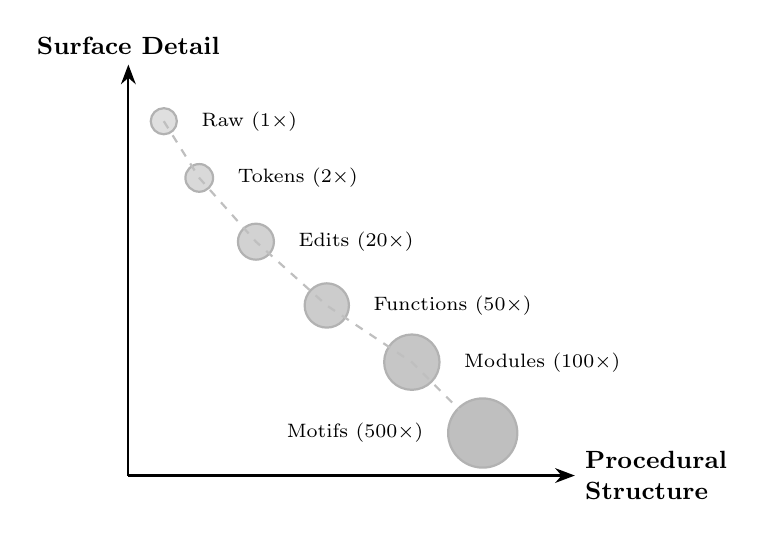
\begin{tikzpicture}[
    scale=0.9,
    axis/.style={-{Stealth[length=2.5mm]}, thick},
    rung/.style={circle, draw=black!30, thick},
    runglabel/.style={font=\scriptsize},
    dimlabel/.style={font=\small\bfseries}
]

% Axes
\draw[axis] (0,0) -- (0,5.8) node[above, dimlabel, align=center] {Surface Detail};
\draw[axis] (0,0) -- (6.3,0) node[right, dimlabel, align=left] {Procedural\\Structure};

% Rungs - bubble size shows compression ratio
% Raw
\node[rung, fill=gray!25, minimum size=8pt] (raw) at (0.5, 5.0) {};
\node[runglabel, right=5pt] at (raw.east) {Raw (1$\times$)};

% Tokens
\node[rung, fill=gray!30, minimum size=10pt] (tokens) at (1.0, 4.2) {};
\node[runglabel, right=5pt] at (tokens.east) {Tokens (2$\times$)};

% Edits
\node[rung, fill=gray!35, minimum size=13pt] (edits) at (1.8, 3.3) {};
\node[runglabel, right=5pt] at (edits.east) {Edits (20$\times$)};

% Functions
\node[rung, fill=gray!40, minimum size=16pt] (functions) at (2.8, 2.4) {};
\node[runglabel, right=5pt] at (functions.east) {Functions (50$\times$)};

% Modules
\node[rung, fill=gray!45, minimum size=20pt] (modules) at (4.0, 1.6) {};
\node[runglabel, right=5pt] at (modules.east) {Modules (100$\times$)};

% Motifs
\node[rung, fill=gray!50, minimum size=25pt] (motifs) at (5.0, 0.6) {};
\node[runglabel, left=5pt] at (motifs.west) {Motifs (500$\times$)};

% Connecting line
\draw[dashed, gray!50, line width=0.8pt] 
    (raw.center) -- (tokens.center) -- (edits.center) -- 
    (functions.center) -- (modules.center) -- (motifs.center);

\end{tikzpicture}
\Description[Representation dimensions visualization]{A two-dimensional plot showing six representation rungs (Raw, Tokens, Edits, Functions, Modules, Motifs) positioned along axes of Surface Detail (vertical) and Procedural Structure (horizontal). Bubble size increases with compression ratio from 1x (Raw) to 500x (Motifs). A dashed line connects all rungs showing the progression from high surface detail to high procedural structure.}
\caption{Representation dimensions. Each rung captures a different aspect of developer workspaces. Bubble size indicates compression ratio. Higher rungs collapse surface detail (vertical) while preserving procedural structure (horizontal).}
\label{fig:rung_dimensions}
\end{figure}

\section{Abstractions makes evaluating workflows tractable}
\label{sec:evaluation}

\textbf{Representations make workflows measurable and comparable.} Representations turn workflows into objects that can be measured, compared, and optimized. We define two complementary quantities: \emph{intra-trace similarity} measures how well a representation preserves information within a single trace (expressiveness), while \emph{inter-trace similarity} measures how similar different traces become after abstraction (identifiability). Higher inter-trace similarity indicates that traces blend together, making them less distinguishable. \textcolor{blue}{The $\varepsilon$-gap = intra-trace similarity - inter-trace similarity measures \emph{identifiability}: how well traces can be distinguished from each other. A large gap means traces remain distinguishable (high expressiveness, high identifiability); a small gap means traces blend together (low expressiveness, low identifiability). This is one dimension of privacy---reconstructability (can the original trace be recovered?) and information leakage (what sensitive data persists?) are separate concerns.}

\textcolor{blue}{Higher rungs reduce identifiability: motifs achieve higher inter-trace similarity (traces blend together), while tokens achieve lower inter-trace similarity (traces remain distinguishable). The $\varepsilon$-gap quantifies identifiability, enabling principled selection of abstraction levels based on privacy requirements.} The representation dimensions also enable searching across workspaces for workflows or programs satisfying specific properties along different dimensions---finding refactoring patterns (motif dimension), similar API evolution (function dimension), or architectural changes (module graph dimension).

\textcolor{blue}{\textbf{Privacy, expressiveness, and utility are three separate dimensions.} Abstraction is usually framed as privacy versus utility. But these are three separate dimensions that do not trade off symmetrically. Higher abstraction can \emph{increase} utility: raw traces are noisy, while motifs expose transferable procedure. A debug loop motif works across Python, TypeScript, and Java; the raw token sequence does not. Privacy has multiple dimensions: the $\epsilon$-gap measures identifiability (can traces be distinguished?), while reconstructability (can the original trace be recovered?) and information leakage (what sensitive data persists?) are separate. Organizations select rungs based on which privacy dimension matters most: compliance may require low reconstructability (motifs), while research may tolerate higher identifiability if leakage is bounded (semantic edits with canonicalization).}

\textbf{Evaluation becomes comparison of workflows, not final code.} Two models are evaluated by comparing how they work: the patterns of edits they make, how they use context, how they recover from errors, and how they move through a codebase when solving the same kind of problem. Evaluation becomes a comparison of workflows, not just a check on final code.

\textbf{Compression reduces cognitive load.} Abstraction is compression, and compression narrows the focus of an evaluator~\cite{miller1956magical}. A developer reviewing thousands of sessions cannot inspect raw traces; they need representations that surface relevant structure while hiding irrelevant detail~\cite{gero2024sensemaking}. \textcolor{blue}{Higher rungs achieve substantial compression (orders of magnitude) from raw to motifs, reducing cognitive load: at the motif level, a developer sees workflow patterns (test-first, refactor-then-extend) rather than individual keystrokes.}

\textbf{Different rungs suit different tasks.} Tokens support fine-grained debugging and code completion evaluation. Semantic edits support refactoring detection and change impact analysis. Functions support API evolution and interface stability. Module graph supports architectural drift analysis, dependency management, and file-level activity pattern detection. Motifs support workflow classification, procedural search, and governance. \textcolor{blue}{A key application is context retrieval: finding relevant files or code snippets for a prompt across thousands of sessions. Different rungs trade off retrieval performance for privacy: raw traces enable high recall but require full code access; semantic edits enable moderate recall with compression; motifs enable privacy-preserving search but lower recall. Organizations can select rungs based on privacy requirements, trading retrieval performance for privacy as needed.}

Structural patterns generalize better than raw content~\cite{yun2023emergence}. Patterns like discovered intent clusters work across Python, TypeScript, and Java; token sequences are language-specific. The uniqueness ratio drops from raw to motifs, revealing shared underlying structure.

\textbf{Lens-level ablations reveal which signals survive abstraction.} This motivates lens-level ablations: rather than ablating model components, we ablate representational access and measure performance degradation. This reveals which abstractions suffice for which tasks---asking not ``How well does the model perform?'' but ``Which aspects of behavior survive abstraction?''

\textcolor{blue}{\textbf{Evaluation framework: probe-based analysis.} To evaluate which rungs preserve which signals, we use probe-based analysis: train simple linear classifiers on representations to measure predictive signal content. If a probe achieves high accuracy on motifs but low accuracy on tokens, procedural structure survives abstraction while syntactic detail does not. Inter-probe difference---the variance in probe performance across rungs---indicates when rung choice matters versus when all rungs contain similar signal, enabling adaptive rung selection based on task requirements.}

Abstraction is lossy compression, and the privacy--expressiveness trade-off corresponds to an information bottleneck that preserves workflow patterns while discarding code-level detail.

\section{Representations as levers for steering AI-assisted engineering}
\label{sec:steering}

\textbf{Workflows become steerable once represented.} Once workflows are represented, they become steerable. We can define objectives not over outputs but over processes: minimizing unnecessary context churn, encouraging test-driven loops, or limiting cascade edits from fragile configuration files. These constraints act as \emph{regulatory pressures} on development, shaping how agents and humans work together.

\textcolor{blue}{This enables a shift from output governance to process governance. Instead of specifying what code should look like, organizations can specify how development should proceed---encouraging efficient patterns and discouraging antipatterns. The representation layer becomes the interface through which these constraints are expressed and enforced.}

\textbf{Change propagation reveals leverage points.} Beyond abstraction, we analyze how changes propagate through codebases. Modifying file $A$ triggers subsequent changes to files $B$, $C$, $D$, forming directed propagation graphs. These cascades reveal architectural leverage: some files trigger many downstream changes, others are isolated. Understanding propagation patterns guides engineering priorities---identifying fragile dependencies, predicting impact, and optimizing change strategies.

\textcolor{blue}{\textbf{Emergent intents guide research priorities.} Static benchmarks like HumanEval remain useful for measuring output correctness, but they cannot identify which \emph{workflow patterns} correlate with success. Just as Clio used clustering to discover high-leverage conversation patterns, emergent intent discovery reveals which procedural strategies succeed at fine granularity. Clustering metrics (completeness, homogeneity, boundary quality) validate that discovered categories capture meaningful developer behavior rather than noise. This enables targeted research: instead of asking ``How do we improve code generation?'' we ask ``Which intent patterns correlate with efficient task completion?'' Representations make these questions empirically tractable, guiding research toward highest-leverage interventions.}

This shifts the locus of control from code to procedure. Instead of telling models what to write, we regulate how work unfolds. Representations become the interface through which software engineering itself is governed.

\section{Aggregating local workflows into collective intelligence}
\label{sec:vision}

\textbf{High-level abstractions enable collective learning.} The long-term goal is a shared substrate for learning from real software development while preserving privacy. High-level abstractions can be safely shared across users and organizations, enabling collective intelligence about how effective development happens in practice. \textcolor{blue}{Just as humans converge on shared procedural abstractions through collaboration~\cite{mccarthy2021learning}, developers and agents can build a common vocabulary of effective strategies through aggregated motif distributions.} \textcolor{blue}{Recent work on information design for collaborative platforms~\cite{haghtalab2024platforms} shows that platforms with information advantages can structure signals to steer strategic agents toward efficient collaboration. The representation layer provides such an advantage: by abstracting workflow patterns, the platform can reveal aggregate insights (efficient motif distributions, successful strategies) while preserving individual privacy, addressing the incentive alignment problem that often undermines collaborative systems.}

\textbf{Three missing capabilities become possible.} This unlocks three capabilities that are currently missing: (1) the ability to evaluate code agents based on how they perform real software engineering work across different environments, (2) a shared language for analyzing and comparing workflows at scale, and (3) the ability to aggregate and learn from these patterns while preserving developer privacy.

\textcolor{blue}{\textbf{Representations enable bidirectional alignment.} A new programming paradigm is emerging where developers orchestrate agents through declarative specifications---DSLs that compile to model calls, protocols that standardize tool access. But current orchestration is blind: developers choose models based on benchmark scores, not procedural fit. Workflow representations enable bidirectional alignment: (1) \emph{Aligning AI to developer needs}---by measuring how different models work (their motif distributions, error recovery patterns, context management strategies), we can match models to tasks empirically. A model that excels at ``plan-then-implement'' motifs may suit greenfield features; one with tight debug loops may suit bug fixes. (2) \emph{Aligning developers to AI capabilities}---representations reveal which procedural strategies succeed, helping developers understand which workflows work best with different AI systems. This bidirectional alignment preserves human agency: developers learn which strategies are effective while maintaining control over orchestration decisions. Representations become the interface through which both directions of alignment are achieved.}

By making workflows measurable, representations turn everyday development into a continuous evaluation and learning process. This is the foundation for AI systems that do not merely write code, but improve how software is made.

\section{Discussion}

\textbf{Implications for evaluation and learning.} This work demonstrates that learning from program traces in the wild is possible. Workflows exhibit network properties that provide vocabulary for understanding how development unfolds. Abstraction trades expressiveness for privacy in predictable ways: higher rungs achieve substantial compression while preserving structural patterns that generalize across languages where token sequences do not. Different abstraction levels reveal different causal chains: motifs show pattern to task type relationships, semantic edits show edit sequence to workflow relationships, functions show pattern to code organization relationships.

\textbf{Workflow representations enable closed-loop evaluation.} Current benchmarks evaluate code after the fact. They measure whether a model produced a correct solution, not how it worked or whether the process was efficient, recoverable, or extensible. Workflow representations change this. They make development measurable while it happens. This enables a closed loop: representations extracted in real-time can surface inefficiencies (excessive revision cycles, fragile context selection, cascading edits from unstable files). These signals can feed back into behavior. Agents can be constrained by workflow objectives, not just output correctness. Developers can see which strategies succeed before committing to them. Evaluation becomes concurrent with development rather than external to it.

\textbf{Procedural structure may persist under compression.} Prior work has shown that sequence models develop abstract state representations even when intermediate observations are withheld~\cite{yun2023emergence}. Workflow abstractions may behave similarly: encoding task-relevant signals despite compressing surface detail. Probing offers a methodology to test this. If procedural structure persists at high compression while syntax does not, representations have learned to separate strategy from surface.

\textcolor{blue}{\textbf{Motifs as training signal.} Current agent training asks: did it produce correct code? Motif-aware training adds: did it follow efficient procedures? This distinction matters when agents must be interpretable, recoverable, or supervised---\emph{how} a problem is solved affects whether humans can understand, correct, or trust the process.}

\textcolor{blue}{\textbf{Limitations and assumptions.} This framework makes several assumptions. First, it assumes that procedural patterns are learnable and transferable across contexts---that a debug loop in Python shares structure with one in TypeScript. Second, it assumes that abstraction preserves the signals needed for downstream tasks, which may not hold for all applications. Third, it assumes that developers are willing to share workflow data at some abstraction level, which depends on trust and privacy guarantees. Fourth, the framework requires sufficient telemetry coverage to extract meaningful patterns---sparse or noisy traces may yield unreliable representations. Finally, the approach assumes that workflow quality can be measured independently of task outcomes, which may not hold for exploratory or creative work where the process itself is the goal.}

\section{Conclusion}

In this paper, we argue that the next generation of AI evaluation must move from static benchmarks to \emph{in-vivo} measurement of real developer--agent workflows. We introduce a companion system that captures fine-grained Cursor telemetry and propose representation dimensions that transform raw logs into structured abstractions---files, motifs, and context flows---that enable \emph{evals in the wild}. These representations make it possible to measure, compare, and optimize how software is produced, not just what code is output. We demonstrate that abstraction trades expressiveness for privacy in predictable ways, with higher rungs achieving substantial compression while preserving structural patterns that generalize across languages where token sequences do not. We outline how this substrate supports personalization, collective learning, and governance of AI-assisted software engineering.

A number of open questions remain at multiple levels. At the representation level: what is the minimum abstraction that preserves a given class of patterns? Can we design rungs optimized for specific tasks while maintaining privacy? \textcolor{blue}{Can we distinguish stable procedural preferences from situational responses? How do emergent intent clusters evolve over time---do they stabilize, drift with tooling changes, or converge across populations?} At the learning level: can we learn procedural templates encoding engineering constraints independent of syntax? Do motifs transfer across languages, teams, or domains? \textcolor{blue}{Do agent workflows converge toward common patterns, or do they diverge based on user populations?} \textcolor{blue}{Future work could explore deep sequential representation learning (RNNs, LSTMs, Transformers) on event sequences to learn richer temporal dependencies than current grammar-based methods.} At the systems level: can we detect when developers shift between exploration, implementation, and debugging, and adapt abstraction accordingly? What open protocols would enable federated learning over workflows without centralizing traces? \textcolor{blue}{Can procedural profiles become portable across tools and organizations?} And at the evaluation level: what constitutes good workflow? How do we define quality when developers pursue diverse goals?

Representations make workflows measurable. Closed-loop evaluation makes them steerable. The path forward requires answering which abstractions preserve which signals for which purposes. As AI-assisted development becomes ubiquitous, the ability to learn from real workflows---not just static artifacts---will determine whether we can build systems that improve how software is made, not merely how quickly code is generated.

%%
%% The next two lines define the bibliography style to be used, and
%% the bibliography file.
\bibliographystyle{ACM-Reference-Format}
\bibliography{references}

\end{document}

